\section{Performance}
\label{sec:performance}

% The performance of Brel is an important aspect of its evaluation.
% This section will evaluate Brel's performance by measuring the time it takes to load and extract data from XBRL reports.
% The performance of Brel is not part of the requirements set by this thesis.
% However, it serves as an important metric for future versions of Brel to compare their performance against this initial version of Brel.
Assessing Brel's performance is one aspect of its evaluation.
This section will gauge Brel's efficiency by timing the loading processes of XBRL reports.
Although not a primary thesis requirement, this performance analysis
provides a valuable benchmark for future Brel versions.

\subsection{Methodology}

% To measure the performance of Brel, we will use the same set of XBRL reports that we used to evaluate Brel's robustness.
% We will compare the time it takes to load these reports. 
% We will compare these times to the loading and extraction times of the same reports using the XBRL viewer Arelle\cite{arelle}.
% Arelle provides a reasonably accurate comparison to Brel, as it is a mature and widely used XBRL viewer and is also written in Python.
% We will ensure that both Arelle and Brel only operate on local files to avoid network latency.
% This is achieved by running both Brel and Arelle eleven times for each report and taking the average of the last ten runs.
% Since both Brel and Arelle cache the DTSs of the reports, only the first run will include the time it takes to load the DTSs.
% Arelle and Brel both load XBRL reports eagerly, meaning that they load the entire report into memory before extracting any data from it.
% Therefore the time it takes to load the report is a good proxy for the time it takes to extract data from the report.

% We will use the same machine to run both Brel and Arelle.
% A summary of the machine's specifications is shown in table \ref{tab:machine-specs}.
% The full specifications of the machine are available on the Dell website
% \footnote{\url{https://www.dell.com/en-in/shop/laptops-2-in-1-pcs/xps-15-laptop/spd/xps-15-9560-laptop}}.
To assess Brel's performance, the same XBRL reports used in the robustness evaluation will be employed.
We will compare the time required to load these reports in Brel
with that of the XBRL viewer Arelle\cite{arelle}.
Arelle, which is also written in Python,
offers a reliable basis for comparison with Brel, given its maturity and widespread use.
To eliminate network latency, both Brel and Arelle will process only local files.
Each tool will run eleven times on each report, with the average time of the last ten runs being recorded.
This approach accounts for the caching of the DTSs by both tools,
excluding the initial DTS loading time from subsequent runs.
Since Brel and Arelle both employ eager loading of XBRL reports,
the loading time effectively represents the data extraction time.

Both Brel and Arelle will be run on the same computer,
with its specifications summarized in table \ref{tab:machine-specs}.
Complete details of the machine are available on the Dell website\cite{dell_xps_9560_specs}.
% \footnote{\url{https://www.dell.com/en-in/shop/laptops-2-in-1-pcs/xps-15-laptop/spd/xps-15-9560-laptop}}.

\begin{table}[H]
    \centering
    \small
    \begin{tabular}{|l|l|}
        \hline
        \textbf{Component} & \textbf{Specification} \\
        \hline
        System & Dell XPS 15 9560 \\
        CPU & Intel Core i7-7700HQ (4 cores, 8 threads) \\
        RAM & 16 GB (DDR4 2400 MHz) \\
        Storage & 512 GB NVMe SSD \\
        OS & EndeavourOS 2023.08.05 Linux 6.1.55-1-lts \\
        \hline
    \end{tabular}
    \caption{Machine specifications\cite{dell_xps_9560_specs}}
    \label{tab:machine-specs}
\end{table}

% Both Brel and Arelle will be run with the same configuration.
% The configuration is as follows:

% \begin{itemize}
%     \item \textbf{Brel}: Brel version 0.8.0a8
%     \item \textbf{Arelle}: Arelle version 2.15.0
%     \item \textbf{Python}: Python 3.11.5
% \end{itemize}

% We will use the CLI of Arelle version 2.15.0 to load the reports.
% Conversely, we will use the \text{viewer.py} outlined in section \ref{sec:usability} to load the reports using Brel version 0.8.0a8.
% Both Brel and Arelle will be run on Python 3.11.5 on the same machine in separate shells.
% Arelle will be run with the following command:

The table \ref{tab:software-versions} shows the versions of the software used in the performance evaluation.

\begin{table}[H]
    \small
    \centering
    \begin{tabular}{|l|l|}
        \hline
        \textbf{Software} & \textbf{Version} \\
        \hline
        Brel & 0.8.0a8 \\
        Arelle & 2.15.0 \\
        Python & 3.11.5 \\
        \hline
    \end{tabular}
    \caption{Software versions}
    \label{tab:software-versions}
\end{table}

Both Brel and Arelle\footnote{\url{https://github.com/Arelle/Arelle/releases/tag/2.15.0}} will be run with the same configuration in separate shells.
Arelle will be run with the following command:

\begin{lstlisting}[language=bash, basicstyle=\ttfamily\small]
python arelleCmdLine.py -f /path/to/report.xml
\end{lstlisting}

% Brel will be run with the following command:
% Brel will re-use the same CLI tool that we used to evaluate Brel's usability.
% Whilst Brel will be run with the following command:
Brel will use the \texttt{viewer.py} script outlined in section \ref{sec:usability}.

\begin{lstlisting}[language=bash, basicstyle=\ttfamily\small]
python viewer.py /path/to/report.xml
\end{lstlisting}

\subsection{Results}

% The results of the performance evaluation are shown in figure \ref{fig:performance}.
% The plot shows the average loading time against the number of facts in the report for both Brel and Arelle.
% The number of facts in the report is a good proxy for the size of the report.
% Both the time and the number of facts are plotted on a logarithmic scale.
% Each point on the plot represents the average loading time of a report with a certain number of facts.
% The lines next to the points represent the standard deviation of the loading times for each report.
The outcomes of the performance evaluation are depicted in figure \ref{fig:performance}.  
This figure illustrates the average loading times in relation to the number of facts in each report for both Brel and Arelle.  
The count of facts in each report serves as an effective measure of the report's size.  
In the plot, both the loading times and the number of facts are represented on logarithmic scales.  
Each data point on the plot corresponds to the average loading time for a report containing a specific number of facts.  
Adjacent to these points, lines are shown, indicating the standard deviation of loading times for each report.

\begin{figure}[H]
    \centering
    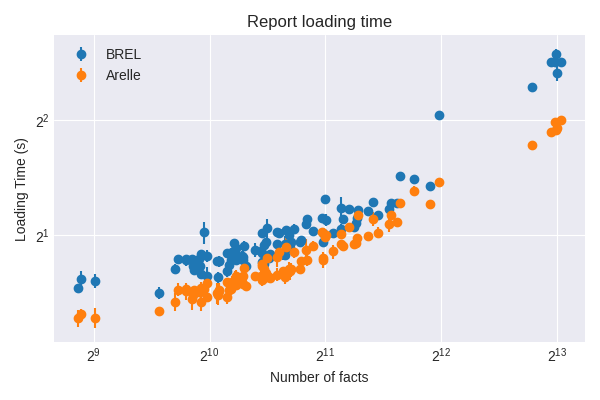
\includegraphics[width=\textwidth]{images/performance_graph.png}
    \caption{Performance of Brel and Arelle}
    \label{fig:performance}
\end{figure}

% The performance test includes 97 reports, whereas each report is run 11 times for both Brel and Arelle
% \footnote{The 3 missing reports are from Thermo Fisher Scientific and The Walt Disney Company, which were not listed on the SEC website at the time of the performance test.}.
% On average, Arelle takes 18\% less time than Brel to load the same report.
% The average time it takes to load a report with Brel is 2.17 seconds, while Arelle takes 1.81 seconds.
The performance evaluation encompassed 97 reports, each tested ten times using both Brel and Arelle\footnote{The 3 missing reports are from Thermo Fisher Scientific and The Walt Disney Company, which were not available on the SEC website during the performance test.}.
On average, Arelle demonstrates an 18.5\% faster loading time than Brel for the same reports.
Brel's average loading time for a report is 2.17 seconds, compared to Arelle's 1.81 seconds.

% The standard deviation of the loading times for both Brel and Arelle is 0.05 seconds.
% This means that the loading times of both Brel and Arelle are consistent across different runs.
% The standard deviation of the loading times is also consistent across different reports with a few exceptions.
% These exceptions can most likely be attributed to the machine's background processes and are not significant enough to affect the overall performance of Brel and Arelle.
Both Brel and Arelle exhibit a standard deviation in loading times of 0.05 seconds.
This consistency in loading times is evident across different runs for both tools.
The standard deviation remains constant across various reports, with a few exceptions.
These outliers are likely due to background processes on the machine and do not significantly impact Brel's or Arelle's overall performance.
% The loading time difference between Brel and Arelle is statistically significant\footnote{Based on a p-value of 0.05}.
Based on a p-value of 0.05, we can statistically confirm the significant difference in loading times between Brel and Arelle.

% \subsection{Discussion}

% The performance of Brel is satisfactory.
% However, the difference in loading times between Brel and Arelle is statistically significant
% \footnote{Assuming a p-value of 0.05}.

% From a qualitative perspective, the report loading times of both Brel and Arelle are acceptable,
% as they are significantly faster than the time it takes to download all files necessary to load the report.
% In general, the download time of the report is the bottleneck in the process of loading an XBRL report.
% Downloading a report tends to be in the order of tens of seconds, while loading the report is in the order of seconds.
% This discussion on download times is deliberately kept vague, as download times are highly dependent on the user's internet connection and the size of the report.

From a qualitative standpoint, the loading times for both Brel and Arelle are acceptable,
being significantly shorter than the time required to download the necessary files for report loading.
% Typically, the download phase is the more time-consuming aspect of loading an XBRL report.
Typically, the download phase more significantly impacts the loading process of an XBRL report.
While download durations often span tens of seconds, loading times are generally within a few seconds.
The discussion of download times is intentionally kept vague, as these times vary greatly depending on the user's internet speed and the report's size.

Arelle most likely outperforms Brel due to its maturity and the optimizations it has undergone over the years.
Brel, on the other hand, is still in its early stages of development and has not yet undergone major optimizations.
Brel's XBRL link parser is a prime candidate for optimization, as it is the most time-consuming part of the report loading process.
